\documentclass{article}

\usepackage[utf8]{inputenc}

\usepackage{textcomp}
\usepackage[T1]{fontenc}
\usepackage{multirow}
\usepackage{float}
\usepackage[caption = false]{subfig}
\usepackage{longtable}
\usepackage{listings}
\usepackage{mathtools}
\DeclareMathOperator{\tr}{Tr}
\usepackage{commath}
\usepackage{bbold}
\usepackage{xcolor}
\usepackage{physics}
%\usepackage[margin=1.8cm]{geometry}

\usepackage{tikz-cd}
\usepackage{amsmath}
\usepackage{amsfonts}
\usepackage{amssymb}
\usepackage{amsthm}
\usepackage{graphicx}
\usepackage[colorinlistoftodos]{todonotes}
\usepackage[colorlinks=true, allcolors=blue]{hyperref}
\usepackage{siunitx}
\sisetup{separate-uncertainty=true}

\usepackage[sc]{mathpazo}
\linespread{1.05}         % Palladio needs more leading (space between lines)
\usepackage[T1]{fontenc}

\newcommand{\diag}[1]{\text{diag}\qty(#1)}
\newcommand{\const}{\text{const}}
\newcommand{\sign}[1]{\text{sign}\qty(#1)}
\renewcommand{\H}{\mathcal{H}}
\renewcommand{\dim}{\text{dim}}
\newcommand{\C}{\mathbb{C}}
\newcommand{\R}{\mathbb{R}}
\newcommand{\N}{\mathbb{N}}
\newcommand{\Z}{\mathbb{Z}}

\renewcommand{\var}[1]{\text{var} \qty(#1)}
\newcommand{\average}[1]{\langle #1 \rangle}

\newcommand\mybox[1]{%
  \fbox{\begin{minipage}{0.9\textwidth}#1\end{minipage}}}


\begin{document}

It might be more accurate for the Coulomb term in the SEMF to be proportional to \(Z(Z-1)\), since, modeling the protons as point particles, the proper expression for the energy would be:

\begin{equation} \label{eq:SEMF-coulomb-correction}
    U = \frac{e^2}{4 \pi \varepsilon_0} \sum _{i=1}   ^{Z} \sum _{j<i} \frac{1}{\abs{r_i - r_j} }  \propto \frac{Z(Z-1)}{\abs{\overline{r} } }  \propto \frac{Z(Z-1)}{A^{1/3}}
\end{equation}

where \(\overline{r} \) is the average distance between the protons in the nucleus. We do not know what its expression looks like, but surely \(\overline{r} \propto r _{\text{nucleus}}  \propto A^{1/3}\).

\paragraph{Specular nuclei}

They are pairs of nuclei with odd \(A\) and \(Z\)s equal to \((A \pm 1)/2\).

The only term which changes in the SEMF between them is the Coulomb, therefore (using the modified Coulomb term given in \eqref{eq:SEMF-coulomb-correction}) their difference in energy is given by

\begin{subequations}
\begin{align}
  \Delta B  &= \frac{a_C}{A^{1/3}} \qty(\frac{(A+1)(A-1)}{4} - \frac{(A-1)(A-3)}{4})  \\
  &= \frac{a_C}{A^{1/3}} \qty(\frac{4A -4}{4})  \\
  &= a_C \qty(A^{2/3} - A^{-1/3})
\end{align}
\end{subequations}

With the Coulomb term which models the nucleus as a uniformly charged sphere, \(a_C Z^2 A^{-1/3}\), we get \(\Delta B = a_C A^{2/3}\) instead.

We can plot the data for \(\Delta B\) wrt \(x \defeq A^{2/3}\). The plot will be of the form

\begin{equation} \label{eq:delta-B-options}
    \Delta B  = a_C x - \frac{a_C}{\sqrt{x}} \qquad \text{or} \qquad \Delta B = a_C x
\end{equation}

We fit the two options given in equation \eqref{eq:delta-B-options}: the results are shown in figure \ref{fig:odd-A-fit}.

\begin{figure}[H]
    \centering
    \begin{subfigure}{0.5\textwidth}
        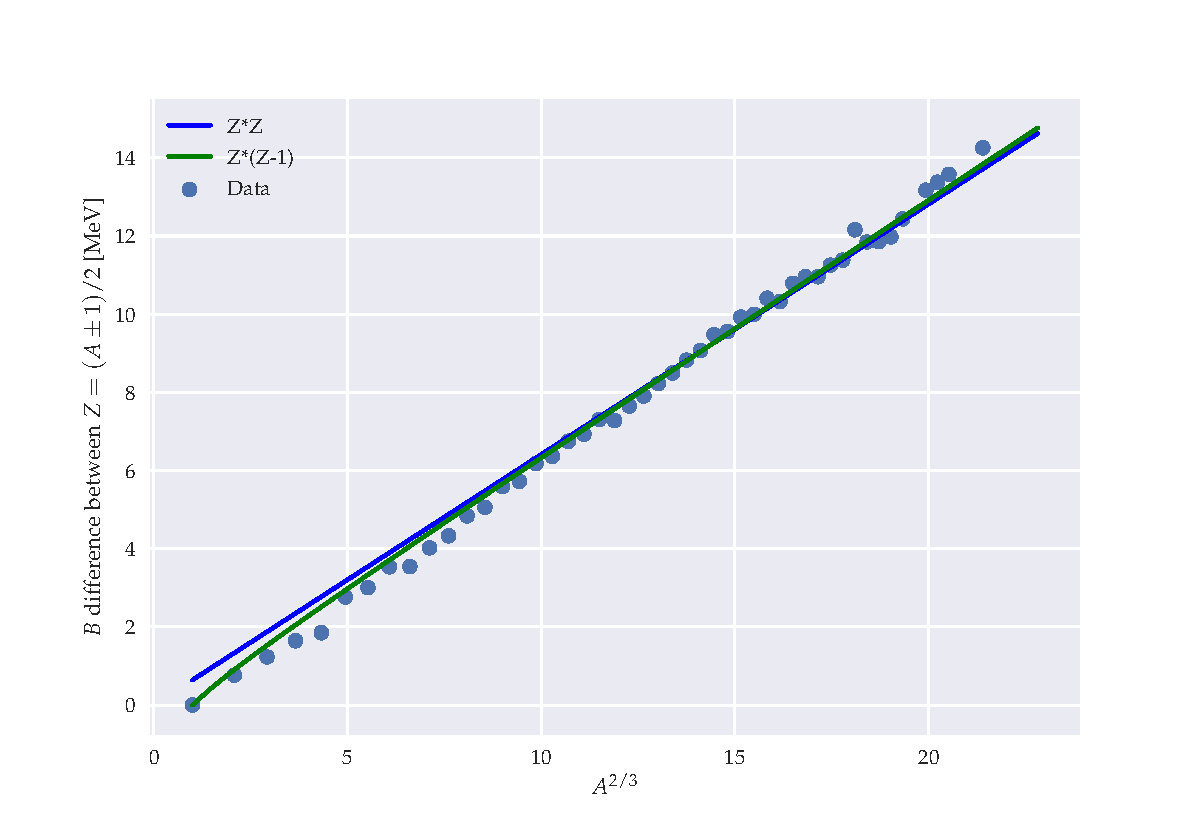
\includegraphics[width=\textwidth]{figures/odd_A_fit.pdf}
        \caption{Fit}
    \end{subfigure}%
    \begin{subfigure}{0.5\textwidth}
        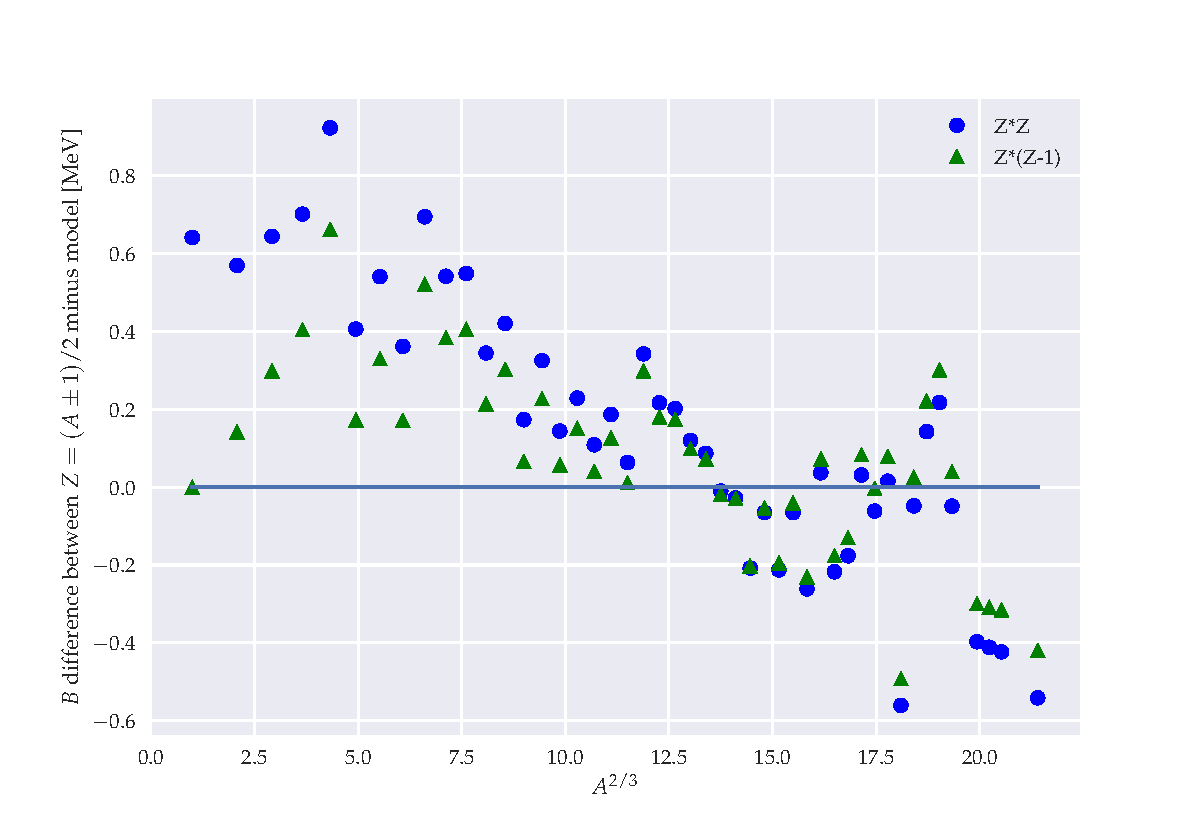
\includegraphics[width=\textwidth]{figures/odd_A_residuals.pdf}
        \caption{Residuals}
    \end{subfigure}%
    \caption{Fit of the difference in \(B\) between symmetric nuclei. The chi square is \(\SI{0.136}{MeV^2} \) for the \(Z^2\) model, and \(\SI{0.062}{MeV^2}\) for the \(Z(Z-1)\) model.}
    \label{fig:odd-A-fit}
\end{figure}


The fit gives us \(a_C = \SI{631(5)}{keV}\) in the new parametrization (the error is only indicative, as I did not have errorbars for the binding energies).

\begin{flushright}
    Jacopo Tissino, 21 june 2019
\end{flushright}


\end{document}
